%===================================== CHAP 7 =================================

\chapter{Project life cycle}
\label{ch:project_lifecycle}

\section{Planning and research}
\label{sec:project_lifecycle-planning_and_research}

This section provides a general description of the planning and research phase of the process. It attempts to capture the main aspects of the process and work done.

\subsection{Planning phase}
\label{subsec:project_lifecycle-planning_and_research-planning_phase}

The planning phase of this project consisted mainly of defining the outer scope of the project. That included negotiating core requirements with the customer, as well as research on relevant technologies and existing solutions. A report document structure was also created, and both the introduction and parts of the prestudies chapter were written. The group also had to define internal meeting and communication terms.

\subsubsection{Goals}
\label{subsec:project_lifecycle-planning_and_research-planning_phase-goals}

\begin{enumerate}
\item Discuss and define the project description.
\item Define core functional requirements.
\item Research previous and similar work.
\item Select development strategy and team organization.
\item Define development and communication environment.
\end{enumerate}

\subsubsection{Discussion}
\label{subsec:project_lifecycle-planning_and_research-planning_phase-discussion}

All of the goals were achieved in this phase. The work required during this phase was somewhat overestimated. This was mainly due to reaching agreement with the customer quickly, and the group working well together from the beginning. In total, 180 hours were spent on the planning phase, out of the 240 hours initially planned. 40 of these hours were dedicated to defining the report structure and writing chapter 1 and 2. The remaining 60 hours could have been used more efficiently. Partn of this time was used to construct the outlines of the report, but the remainder should have been allocated to the research phase. 

\subsection{Research phase}
\label{subsec:project_lifecycle-planning_and_research-research_phase}

The research phase of this project was initially introduced due to the option of using Apollo (see section \ref{subsec:prestudies-existing_solutions-apache_apollo}) as the core of the system. Thus, the only goal of this phase was to do extensive research, and find out whether to expand Apollo or develop a new system. The research work was split into different focal points, in order to assess all the major points of uncertainty (see table \ref{tab:risk_analysis_apollo}). At the end of this phase, a decision had to be made. This was anchored in the risk analysis, and could trigger the group to fall back to the alternative solution.

\subsubsection{Discussion}
\label{subsec:project_lifecycle-planning_and_research-research_phase-discussion}

The group was able to reach a decision regarding the system. The choice was a result of the repeated evaluation of the focal points in the associated risk analysis (see table \ref{tab:risk_analysis_apollo}). Two of the members were able to get a fairly good overview of the Scala programming language. However, problems arose when the code base was thoroughly inspected. It proved to be massive, and it required a lot more research to get a good enough understanding of. That also affected the time it would take to implement additional protocol modules. After hours of discussion, Apollo was ultimately discarded. The following arguments made the basis for the final decision:

\begin{itemize}
\item The group did not have sufficient understanding of the asynchronous workings of the embedded Scala classes
\item Apollo is a fairly large and complex project, that requires a lot of effort to get a complete grasp on.
\item Even though Apollo has a dynamic architecture, allowing extension by adding custom Java archived components, it requires thorough understanding of the core application.
\item The group could not justify proceeding with Apollo, given the time available and the risk of not being able to gain a proper understanding in time to complete a working product.
\end{itemize}

A large amount of time had been invested in this research phase, and one might argue that it impacted the product development in a negative way. This is mainly due to lost development time. The positive aspect of it was that several good practices and ways to implement a brokering system were learned. Additionally, the group might not have been able to finish a working product in time, had the decision been to proceed with Apollo before understanding the amount of knowledge and effort required.

The first chapters of the report were also being written at this stage, and 56 hours were used on this task as well as project management during the research phase.

\section{Development}
\label{subsec:project_lifecycle-development}

This section describes the iterations devoted to development of the software. The following section include a general explanation of each sprint, as well as issues that were faced by the group. With the development phase of the project, burndown charts were introduced. The charts reflect the planned and actual time usage for each sprint. This was made in combination with a list of development tasks to be executed for each sprint. Tasks that were not completed in a sprint were transferred to the next sprint. The tasks functioned as an interpretation of sprint backlogs. They do not directly consider the requirements or user stories, but rather work packages from the development part of the WBS (see section \ref{subsec:process_and_methodology-resource_management-work_breakdown}).  The charts do not consider time used on non-development tasks like the report, peer evaluation and meetings.

\subsection{Sprint 1}
\label{subsec:project_lifecycle-development-sprint_1}

This was the first of the development cycles. It consisted mainly of setting up the development environment, and constructing the base project templates and structure. At the end of the sprint, the goal was to have a solid foundation both for the broker and for the web interface. Additionally, the development methodology were to be documented in the report.

\subsubsection{Goals}
\label{subsec:project_lifecycle-development-sprint_1-goals}

\begin{center}
\begin{table}[ht!]
\small
\centering
\begin{tabular}{|p{10cm}|p{2cm}|}
\hline
\rowcolor{lightgray}
 \textbf{Task} & \textbf{Status} \\
\hline
\rowcolor{green!30}
 Initial JavaScript modules for admin console & Completed  \\
 \rowcolor{green!30}
 Template for admin console & Completed \\ 
 \rowcolor{green!30}
 Web server instance & Completed \\ 
 \rowcolor{green!30}
 Decide on technology stack & Completed \\ 
 \rowcolor{green!30}
 Project structure & Completed \\
 \rowcolor{green!30}
 Create initial core service architecture & Completed \\
 \rowcolor{green!30}
 Initial database design and relational schema & Completed \\
\hline
\end{tabular}
\caption{Goal achievement for sprint 1}
\label{tab:sprint 1, goals}
\end{table}
\end{center}

\begin{center}
  \begin{figure}[htbp!]
    \makebox[\textwidth]{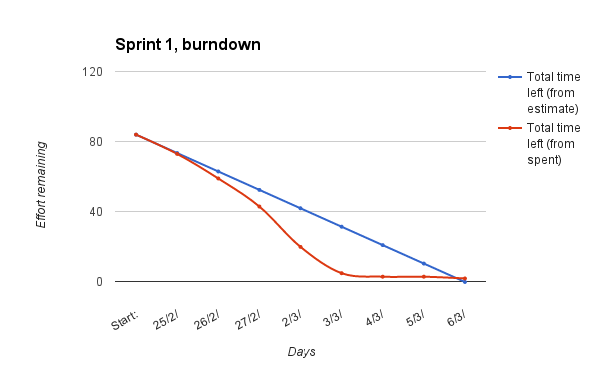
\includegraphics[width=\textwidth]{fig/burndown/sprint1Burndown.png}}
    \caption{Burndown chart for sprint 1}
    \label{fig:sprint 1, burndown}
  \end{figure}
\end{center}

\subsubsection{Discussion}
\label{subsec:project_lifecycle-development-sprint_1-discussion}

As expected, the first development sprint was fairly straightforward. The structure of the project was strongly influenced by Apollo. That made the work of defining the structure and base templates simpler, and less time consuming than first expected. There were also some minor deviations in the time spent on tasks versus the time that was estimated, but no specific issues arose at the time. 40 hours were spent on report writing and project management during this sprint.

\subsection{Sprint 2}
\label{subsec:project_lifecycle-development-sprint_2}

The major goals of sprint 2 was to initialize the first draft of the web interface, as well as identify and implement support for processing incoming WSN messages. The midterm report was also due at the end of this sprint.

\subsubsection{Goals}
\label{subsec:project_lifecycle-development-sprint_2-goals}

\begin{table}[ht!]
\small
\centering
\begin{tabular}{ | p{10cm} | p{2cm} |}
\hline
\rowcolor{lightgray}
 \textbf{Task} & \textbf{Status} \\
\hline
\rowcolor{orange!40}
Structurize RESTapi & Not completed \\
\rowcolor{green!30}
Mockup for topics pane & Completed \\
\rowcolor{green!30}
JavaScript for creating tables for each topic the broker has a subscription on & Completed \\
\rowcolor{green!30}
Models for topics/stats & Completed \\
\rowcolor{orange!40}
Stats functionality	& Not completed \\
\rowcolor{green!30}
Identify WS-Nu components needed to intercept an incoming message & Completed \\
\rowcolor{orange!40}
Identify WS-Nu components needed to create and deliver a valid WSN soap message & Not completed \\
\rowcolor{orange!40}
Set up the needed components to receive and handle incoming message, and pass it to the CoreService	& Not completed \\
\rowcolor{green!30}
Create initial core service architecture & Completed \\
\hline
\end{tabular}
\caption{Goal achievement for sprint 2}
\label{tab:sprint 2, goals}
\end{table}


\begin{center}
  \begin{figure}[ht!]
    \makebox[\textwidth]{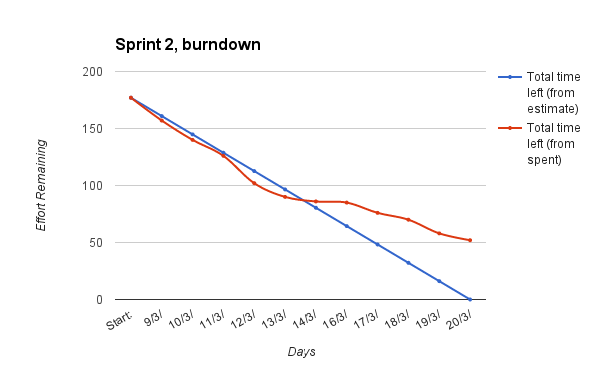
\includegraphics[width=0.9\textwidth]{fig/burndown/sprint2Burndown.png}}
    \caption{Burndown chart for sprint 2}
    \label{fig:sprint 2, burndown}
  \end{figure}
\end{center}

\subsubsection{Discussion}
\label{subsec:project_lifecycle-development-sprint_2-discussion}

At the starting point of this sprint, quite a bit of content lacked on the report in order to deliver a satisfying mid term version. That prompted the group to dedicate a lot of time to the report, and 39 hours were spent on this task. Some of the work regarding WSN had to be pushed to the next sprint along with other, less important, tasks. Obviously, it would have been preferable to finish the work on time. However, quite a lot of time was left before a functional version of the WSN broker was to be completed. Thus, transferring the packages to the next sprint did not cause much concern time-wise. Additionally, the customer seemed happy with the progress, and was satisfied with the topic handling part of the user interface. One group member was ill throughout much of the sprint. This prompted a redistribution of tasks, according to the risk analysis (see section \ref{sec:prestudies-risk_analysis}).

\subsection{Sprint 3}
\label{subsec:project_lifecycle-development-sprint_3}

Only 60 hours of development were initially scheduled for sprint 3. This was due to Easter, and the fact that three of the group members were on a class trip. The main goals of this sprint were topic and subscription mapping. That included both the logic of it, and passing it to the web interface. The incomplete packages from sprint 2 were also included.

\subsubsection{Goals}
\label{subsec:project_lifecycle-development-sprint_3-goals}

\begin{table}[ht!]
\small
\centering
\begin{tabular}{ | p{10cm} | p{2cm} |}
\hline
\rowcolor{lightgray}
 \textbf{Task} & \textbf{Status} \\
\hline
\rowcolor{orange!40}
Create mockup for config pane, including topic mapping & Not completed \\
\rowcolor{green!30}
Structurize RESTapi & Completed \\
\rowcolor{orange!40}
Stats functionality & Not completed \\
\rowcolor{green!30}
Identify WS-Nu components needed to create and deliver a valid WSN soap message & Completed \\
\rowcolor{orange!40}
Set up the needed components to receive and handle incoming message, and pass it to the CoreService & Not completed \\
\rowcolor{orange!40}
Subscription & Not completed \\
\hline
\end{tabular}
\caption{Goal achievement for sprint 3}
\label{tab:sprint 3, goals}
\end{table}

\begin{center}
  \begin{figure}[ht!]
    \makebox[\textwidth]{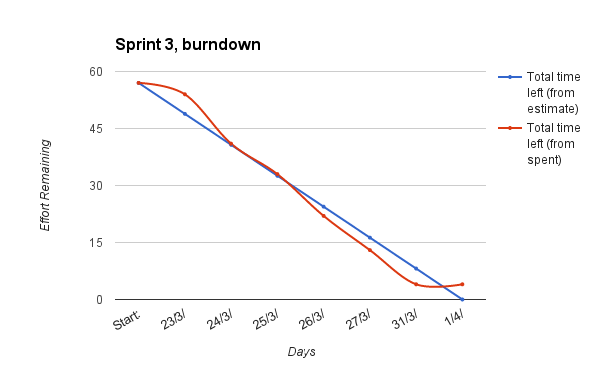
\includegraphics[width=\textwidth]{fig/burndown/sprint3Burndown.png}}
    \caption{Burndown chart for sprint 3}
    \label{fig:sprint 3, burndown}
  \end{figure}
\end{center}

\subsubsection{Discussion}
\label{subsec:project_lifecycle-development-sprint_3-discussion}

At this point, the progress and status of the project was not ideal. After the sprint, some of the smaller packages were still unfinished. They were left untouched due to the importance of the other parts of the system. As the system was shaping up as quite complex, more time was used to identify where and how to implement the different parts. This was obviously an issue, as it decreased the amount of code being added. 20 hours were also used on refining the first chapters of the report, which might have been a bad choice considering the shortcomings in development. However, the subscription and topic handling were almost completed at the end of the sprint. Thus, no remedial actions were taken at the time, but the issues were kept in mind. 


\subsection{Sprint 4}
\label{subsec:project_lifecycle-development-sprint_4}

A lot of work had to be put into the report, the peer evaluation and general research on WSN. The group realized that finishing WSN would be difficult this sprint, so the main focus was to finalize the subscription and publish parts of it. Completing this would be a step in the right direction. The one major issue was deliveries in other courses. This led to little time being scheduled for this sprint. This is something that could have been assessed earlier, and planned for better by following the risk analysis.

\subsubsection{Goals}
\label{subsec:project_lifecycle-development-sprint_4-goals}

\begin{table}[ht!]
\small
\centering
\begin{tabular}{ | p{10cm} | p{2cm} |}
\hline
 \rowcolor{lightgray}
 \textbf{Task} & \textbf{Status} \\
\hline
\rowcolor{green!30}
Create mockup for config pane, including topic mapping & Completed \\
\rowcolor{green!30}
Stats functionality	& Completed \\
\rowcolor{green!30}
Set up the needed components to receive and handle incoming message, and pass it to the CoreService	& Completed \\
\rowcolor{orange!40}
Finish up custom web services and commandproxies that allow interception of requests in WS-Nu	& Not completed \\
\rowcolor{green!30}
Create a first draft of OKSE SubscriptionManager & Completed \\
\rowcolor{green!30}
Create a first draft of OKSE Subscriber and Publisher objects & Completed \\
\rowcolor{orange!40}
Create support methods for transformation to and from WS-Nu request and message representation	& Not completed \\
\rowcolor{green!30}
Create a first draft for OKSE Topic management & Completed \\
\rowcolor{orange!40}
Start looking into MQTT	& Not completed \\
\hline
\end{tabular}
\caption{Goal achievement for sprint 4}
\label{tab:sprint 4, goals}
\end{table}

\begin{center}
  \begin{figure}[ht!]
    \makebox[\textwidth]{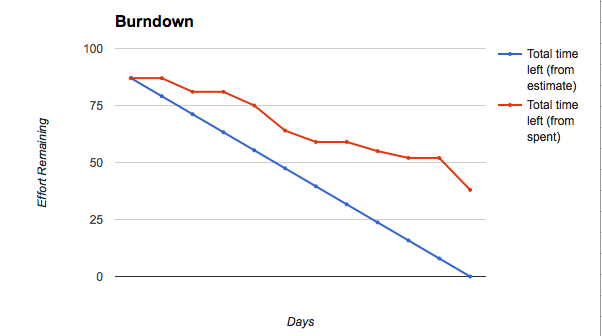
\includegraphics[width=\textwidth]{fig/burndown/sprint4Burndown.png}}
    \caption{Burndown chart for sprint 4}
    \label{fig:sprint 4, burndown}
  \end{figure}
\end{center}

\subsubsection{Discussion}
\label{subsec:project_lifecycle-development-sprint_4-discussion}

The two main reasons for this sprint not containing the planned workload were major deliveries in other courses, as well as group members being in Oslo for summer job interviews. Additionally, 25 hours were spent on the report, which included time spent assessing the mid term feedback. Due to the challenges discussed in the previous sprint, the group had to discuss the priority of requirements with the customer. The solution was to re-prioritize the requirements of MQTT and AMQP support. The result was that AMQP now was the first-in-line protocol to be implemented, pushing MQTT down at a lower priority level. Previously, both AMQP and MQTT had been at the same priority level. That led to a rework of the schedule for the remaining sprints. A lot of time was used for research on the remaining parts of WSN this sprint, along with a lot of report work. WSN proved to be more comprehensive and complex than initially expected, and more code was needed for the implementation than first expected. Even with this in mind, the group still somewhat underperformed. Too little time was dedicated to actual development work. This was an issue, and the solution was to dedicate a lot of time to development the next sprint. A new work plan was made for the remaining sprints (see table \ref{tab:workplan, revised}).


\begin{center}
\begin{table}[ht!]
\centering
\small
\begin{tabular}{ | m{0.4cm} | m{3.3cm}| m{0.7cm} | m{0.9cm} | m{0.9cm}| m{4.4cm} |} 
\hline
\rowcolor{lightgray}
\textbf{ID} & \textbf{Task name} & \textbf{Days} & \textbf{Start} & \textbf{End} & \textbf{Notes} \\
\hline
\textbf{6} & \textbf{Iteration 4} & \textbf{9} & \textbf{07.04} & \textbf{17.04} & \textbf{Monday of Orthodox Easter} \\
 & Stats functionality & & & & \\
 & Subscribe and publish  & & & & \\
\hline
\textbf{7} & \textbf{Iteration 5} & \textbf{9} & \textbf{20.04} & \textbf{30.04} & \textbf{First of May} \\
 & AMQP implementation & & & & \\
 & Finalize WSN & & & & \\
\hline 
\textbf{8} & \textbf{Iteration 6} & \textbf{9} & \textbf{04.05} & \textbf{15.05} & \textbf{Ascension day} \\
 & Finalize AMQP & & & & \\
 & Acceptance test & & & & \\
\hline
\textbf{9} & \textbf{End phase} & \textbf{8} & \textbf{22.05} & \textbf{30.05} & \\
 & Documentation & & & & \\
 & System test & & & & \\
 & \textbf{Delivery} & & \textbf{30.05} & \textbf{30.05} & \textbf{Delivery day} \\
\hline
\end{tabular}
\caption{Updated work plan}
\label{tab:workplan, revised}
\end{table}
\end{center}

\subsection{Sprint 5}
\label{subsec:project_lifecycle-development-sprint_5}
At the start of sprint 5, lectures and tasks were completed in other courses. That meant that all resources could be devoted to the project. Considering the issues explained in the previous sprint, as well as the fact that the time left was getting short, a lot of work was scheduled for this sprint. Extra work hours were introduced in the evenings to assess the lack of time, in accordance with the risk analysis. The main task for this sprint was finalizing the most important aspects of WSN, as well as getting an overview of, and start implementing AMQP support.

\subsubsection{Goals}
\label{subsec:project_lifecycle-development-sprint_5-goals}

\begin{table}[ht!]
\small
\centering
\begin{tabular}{ | p{10cm} | p{2cm} |}
\hline
 \rowcolor{lightgray}
 \textbf{Task} & \textbf{Status} \\
\hline
\rowcolor{green!30}
Create support methods for transformation to and from WS-Nu request and message representation & Completed \\
\rowcolor{green!30}
Get an overview of AMQP standard & Completed \\
\rowcolor{green!30}
Create WSNRegistrationManager class and implement needed methods & Completed \\
\rowcolor{orange!40}
Research, implement and test support and features needed for WSN to use different dialects	& Not completed \\
\rowcolor{orange!40}
Start on writing the developer manual & Not completed \\
\rowcolor{orange!40}
Improve source code documentation & Not completed \\
\rowcolor{orange!40}
Perform component testing of WSNotification	& Not completed \\
\rowcolor{orange!40}
Create subscribers-pane	& Not completed \\
\rowcolor{green!30}
Refactor and improve UI responsiveness & Completed \\
\rowcolor{green!30}
Update GUI to new methods in CoreService & Completed \\
\rowcolor{green!30}
AMQP sendMessage & Completed \\
\rowcolor{green!30}
Refactorization of JS & Completed \\
\rowcolor{orange!40}
AMQP subscribe & Not completed \\
\rowcolor{green!30}
AMQP Driver.stop() & Completed \\
\hline
\end{tabular}
\caption{Goal achievement for sprint 5}
\label{tab:sprint 5, goals}
\end{table}

\begin{center}
  \begin{figure}[ht!]
    \makebox[\textwidth]{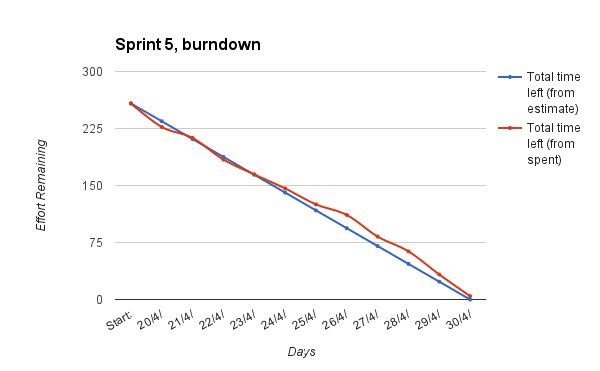
\includegraphics[width=\textwidth]{fig/burndown/sprint5Burndown.png}}
    \caption{Burndown chart for sprint 5}
    \label{fig:sprint 5, burndown}
  \end{figure}
\end{center}


\subsubsection{Discussion}
\label{subsec:project_lifecycle-development-sprint_5-discussion}

Almost all resources were assigned to implementation this sprint, and a lot of work was done on the system. Although a fair amount of the packages were not fully completed at the end, WSN only lacked proper testing before completion. A lot of work had also been done on AMQP, and the protocol proved much simpler than WSN. Thus, the project was almost back on schedule, and it seemed likely that the implementation would be completed after the next sprint. It did, however, seem unlikely that there was sufficient time to implement MQTT. Thus, MQTT was completely abandoned during the group meeting at the end of the sprint, with compliance from the customer. The group noted that research done on the MQTT protocol, and libraries of interest should be documented in the report regardless.

\subsection{Sprint 6}
\label{subsec:project_lifecycle-development-sprint_6}

This was the final period of development. Only a small amount of development work remained before completion of the product. That, along with testing and a lot of report writing were the most important aspects of the sprint. The plan was to finish up the development at the beginning of the sprints, and work on testing and report writing after that. The final days of this sprint had to be dedicated to studying for exams in other courses.

\clearpage

\subsubsection{Goals}
\label{subsec:project_lifecycle-development-sprint_6-goals}

\begin{table}[ht!]
\small
\centering
\begin{tabular}{ | p{10cm} | p{2cm} |}
\hline
\rowcolor{lightgray}
\textbf{Task} & \textbf{Status} \\
\hline
\rowcolor{green!30}
Create subscribers pane & Completed \\
\rowcolor{green!30}
Research, implement and test support and features needed for WSN to use different dialects & Completed \\
\rowcolor{green!30}
Create support for Topic Mapping in TopicService and MessageService & Completed \\
\rowcolor{green!30}
Hook Topic Mapping support up to admin panel & Completed \\\rowcolor{green!30}
AMQP subscribe & Completed \\
\rowcolor{green!30}
AMQP get client port number & Completed \\
\rowcolor{green!30}
Database prepared statements & Completed \\
\rowcolor{green!30}
Graceful shutdown of AMQPProtocolServer & Completed \\
\rowcolor{green!30}
Create UI for relay functionality & Completed \\
\rowcolor{green!30}
Implement functionality for changing password & Completed \\
\rowcolor{green!30}
Improve source code documentation & Completed \\
\rowcolor{green!30}
Perform component testing of WSNotification & Completed \\
\rowcolor{green!30}
Perform component testing of AMQP & Completed \\
\rowcolor{green!30}
Test functionality for graceful shutdown and restart & Completed \\
\hline
\end{tabular}
\caption{Goal achievement for sprint 6}
\label{tab:sprint 6, goals}
\end{table}

\begin{center}
  \begin{figure}[ht!]
    \makebox[\textwidth]{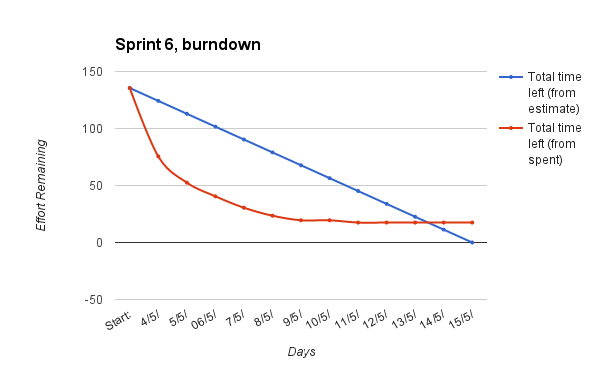
\includegraphics[width=\textwidth]{fig/burndown/sprint6Burndown.png}}
    \caption{Burndown chart for sprint 6}
    \label{fig:sprint 6, burndown}
  \end{figure}
\end{center}

\subsubsection{Discussion}
\label{subsec:project_lifecycle-development-sprint_6-discussion}

Having exams coming up, most of the work was done at the beginning of this sprint. All tasks were completed by the end of this sprint, and both AMQP and WSN was implemented at this point. Only minor challenges arose, but were quickly overcome. The major challenges and headaches regarding WSN and AMQP were already resolved during the last sprint. With a clear remaining path, finalizing the last work packages progressed without noteworthy incidents. As the report had to start shaping up, 50 hours were also spent on writing.

\section{Final phase}

The final phase mostly consisted of report writing and documentation. A lot of final work and reviewing had to be done in order to deliver a satisfying report. That included writing the user and development manual, as well as the evaluation of the project. The plan was to finish the report on the May 26. The report would then be handed to a third party for proofreading. The proofreading covered evaluation of structure, semantics and general language. The final delivery deadline was the May 30, at which point the report would be delivered.

The final phase consisted of the tasks listed in table \ref{tab:final_phase-tasks}, as well as the total amount of time spent on each task.

\begin{table}[ht!]
\small
\centering
\begin{tabular}{ | p{10cm} | p{2cm} |}
\hline
\rowcolor{lightgray}
\textbf{Task} & \textbf{Time Used} \\
\hline
Final system testing and documentation of results & 28 \\
Project evaluation & 30 \\
Report writing & 111 \\
Creating the user manual & 13 \\
Creating the developer manual & 16 \\
Internal report proofreading and reference checking & 22 \\
\hline \hline
Sum & 220 \\
\hline
\end{tabular}
\caption{Tasks and resource usage for the final phase}
\label{tab:final_phase-tasks}
\end{table}

\subsubsection{Discussion}

As the final deadline approached, the group had to put in a large effort to finalize the formal parts of the project. The most prominent part was dedicated to the main report, focusing on the formulation of sentences, syntax, overall structure and readability. Additionally, the group put much effort into evaluating the project as a whole. This had to be done both to summarize lessons learned throughout the project, as well as documenting product related findings to the customer.

An additional task during the final phase was to perform one final system test including all the stated requirements, as well as additional tests of the product. The main reason being that the group had to assure that the results provided were consistent with the behaviour of the system after development had ended. As some flaws were discovered during development, it was also important to check if they were still reproducible, and in any case documented accordingly. This task was performed based on the plan outlined in section \ref{subsec:testing-test_execution-system_testing}.
